\section{Degenerate Gas}

\emph{Kittel \& Kroemer: Chapter 7}
\begin{itemize}
    \item Using Fermi-Dirac Distribution in the low temperature limit
    \item How to use zero temperature Fermi-Dirac Distribution to find expectation values
\end{itemize}

Whenever $n \geq n_Q$ the gas is said to be in the quantum regime, which occurs at high density or low temperature. This is when there are more particles than available states at a given temperature. This is often called a \textbf{degenerate gas}\footnote{Otherwise called "zero-temperature gas", "ground state", or simply "fermi gas".}. The applications of this theory include:
\begin{itemize}
    \item conduction electrons in metals\footnote{This is most familiar to people most likely. I work in this area so am a bit biased towards this application.}
    \item white dwarf stars
    \item liquid $^3$He
    \item nuclear matter
    \item phonons in solids
\end{itemize}
I do not like Kittel's treatment very much, but Dr. Townsley gave good notes in lecture. I highly recommend learning about Bose-Einstein condensates from the book or elsewhere since the class did not get to it. This concept is a big deal in some areas of physics (like Cooper pairs in Type I Superconductors).

\textbf{Fermi Energy:} This concept is revisited in this context. The energy of the highest filled orbital in the ground state of a free particle gas of fermions (will be given to us on exam) is
\[
\epsilon_F = \frac{\hbar^2}{2M} \bigg( \frac{3\pi^2N}{V} \bigg)^{2/3}
\]
Which can be used to find the total kinetic energy in the ground state as 
\[
U_0 = \frac{3}{5} N \epsilon_F
\]

\textbf{Fermi Temperature:} $\tau_F = \epsilon_F$

\textbf{Fermi Occupancy:} $n_F$ is the value of $n$ in the expression of $\epsilon_F$
\begin{figure}[!hbtp]
    \centering
    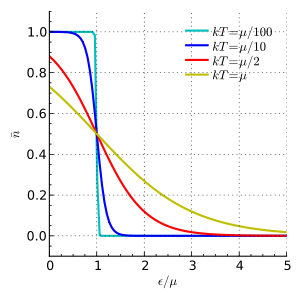
\includegraphics[scale=.2645]{Images/FD-dis.png}
    \caption{Behavior of Fermi-Dirac distribution at different temperatures.}
    \label{fig:fd-dis}
\end{figure}

\newpage
\textbf{Derivation from class:}
The energy of an un-bound electron in a "box" is 
\[
\epsilon_n = \frac{\hbar^2\pi^2}{2mL^2} n^2
\]

We want the Average Occupancy $\langle N \rangle$. This is given by the sum of the Fermi-Dirac Distribution over all energies. This sum can be turned into an integral if the gaps between energy values is small enough, and a factor of two is added for the spin multiplicity.
\[
\langle N \rangle = \int_{all} f_{FD}(\epsilon) d\epsilon 
= 2 \int_0^{\infty} \int_0^{\infty} \int_0^{\infty} f_{FD}(\epsilon) dn_x dn_y dn_z
\]

One can note that the value of $\epsilon$ only depends on the magnitude of $n$, which lends itself to a conversion into pseudo-spherical coordinates in phase space $dn_x dn_y dn_z \to n^2 sin\theta dn d\theta d\phi$. The quantum numbers are only positive, so the limits of integration correspond to the first octant. This is summarized below.
\[
    \left. \begin{aligned}
        0 \leq n_x \\
        0 \leq n_y \\
        0 \leq n_z
    \end{aligned}
    \right \}
\qquad
\implies
    \left. \begin{aligned}
        0 \leq n \\
        0 \leq \theta \leq \pi/2 \\
        0 \leq \phi \leq \pi/2
    \end{aligned}
    \right \}
\]

The figure above shows how the Fermi-Dirac Distribution approaches the behavior of a step function at zero temperature. This can be written as
\[
f_{FD} = \begin{cases}
            1,  n < n_F \\
            0,  n > n_F
         \end{cases}
\]
Which makes the integral
\[
\langle N \rangle = 2 \int_0^{n_F} \int_0^{\pi/2} \int_0^{\pi/2} f_{FD}(\epsilon) n^2 sin\theta dn d\theta d\phi = \frac{\pi}{3} n_F^3 = N
\]
This can be solved for $n_F = (3N/\pi)^{1/3}$ and put into the $\epsilon_F$ to get it in terms of $N,V$.
\[
\epsilon_F = \frac{\hbar^2}{2M} (3\pi^2)^{2/3} \bigg( \frac{N}{V} \bigg)^{2/3}
\]

Now, to get the expectation value for the energy $\langle U \rangle$, a similar procedure is followed.
\[
\langle U \rangle = 2 \int_0^{\infty} \int_0^{\infty} \int_0^{\infty}  \epsilon(n) f_{FD}(\epsilon) dn_x dn_y dn_z
\]
Using the same change of coordinates
\[
\langle U \rangle = 2 \int_0^{n_F} \int_0^{\pi/2} \int_0^{\pi/2}  \epsilon(n) f_{FD}(\epsilon) n^2 sin\theta dn d\theta d\phi = \frac{\pi^3\hbar^2}{10mL^2} n_F^5
\]
Which becomes the final result
\[
U = \frac{3}{5} N \epsilon_F
\]